%%%%%%%%%%%%%%%%%%%%%%%%%%%%%%%%%%%%%%%%%%%%%%%%%
%%%%%%%%%%%% cap: application %%%%%%%%%%%%%%%%%
%%%%%%%%%%%%%%%%%%%%%%%%%%%%%%%%%%%%%%%%%%%%%%%%%

\chapter{Creating a BCI Application Platform}\label{cap:development}
In this bachelor's thesis, the main objective is creating a BCI App Platform, meaning the creation of a program that can open other applications while interfacing with the Unicorn Hybrid Black, a Brain-Computer Interface, to receive input from a disabled user via a P300 speller. The user can navigate through his favourite applications which are displayed on the platform's graphical user interface using the Unicorn Speller, g.tec's implementation of the P300 speller. Using the speller, he can then select an application to launch and use for as long as he desires, after which he can once again close it through the speller's board by looking at its elements. The results show a stable application that can be used to navigate through compatible apps and open them with ease.

\section{Platform Architecture}
The application to be implemented makes use of a BCI Speller, namely the Unicorn Speller which is part of the Unicorn Suite Hybrid Black. This speller can only be used with the Unicorn Hybrid Black Brain-Computer Interface. The speller is used as the primary and only input method for a disabled user to interact with the application. The BCI headset sends its output (the item the user selected from the board) through a UDP server to a specific IP address and port combo specified in the speller settings. The application implements a UDP listener that runs as a background process of the application, waiting for input from the user. When the aforementioned input arrives, the listener sends it to the application which then interprets it accordingly.
\vspace{\baselineskip}\newline
The platform itself is a Unity application that when run fetches all BCI applications installed on the user's disk and displays them to the user so that he/she can select one. Once an application is selected, the platform simply runs it and locks all user input, as the applications housed inside also interface with the speller and by keeping input unlocked, the user may accidentally open multiple apps or cause other unwanted behaviour.

\begin{figure}[H]
  \centering
  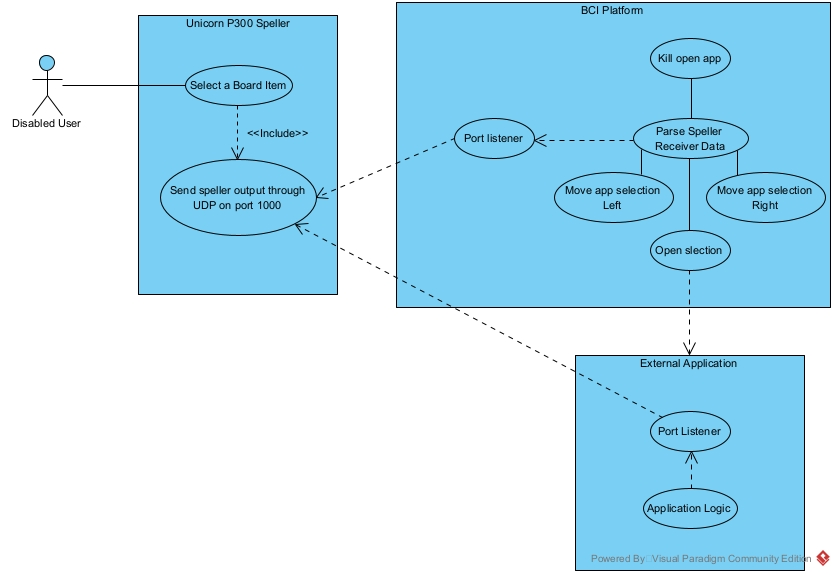
\includegraphics[width=1\textwidth]{Diagrams/Platform Use Case.jpg}
  \caption{Platform use case diagram}
\end{figure}
\begin{figure}[H]
  \centering
  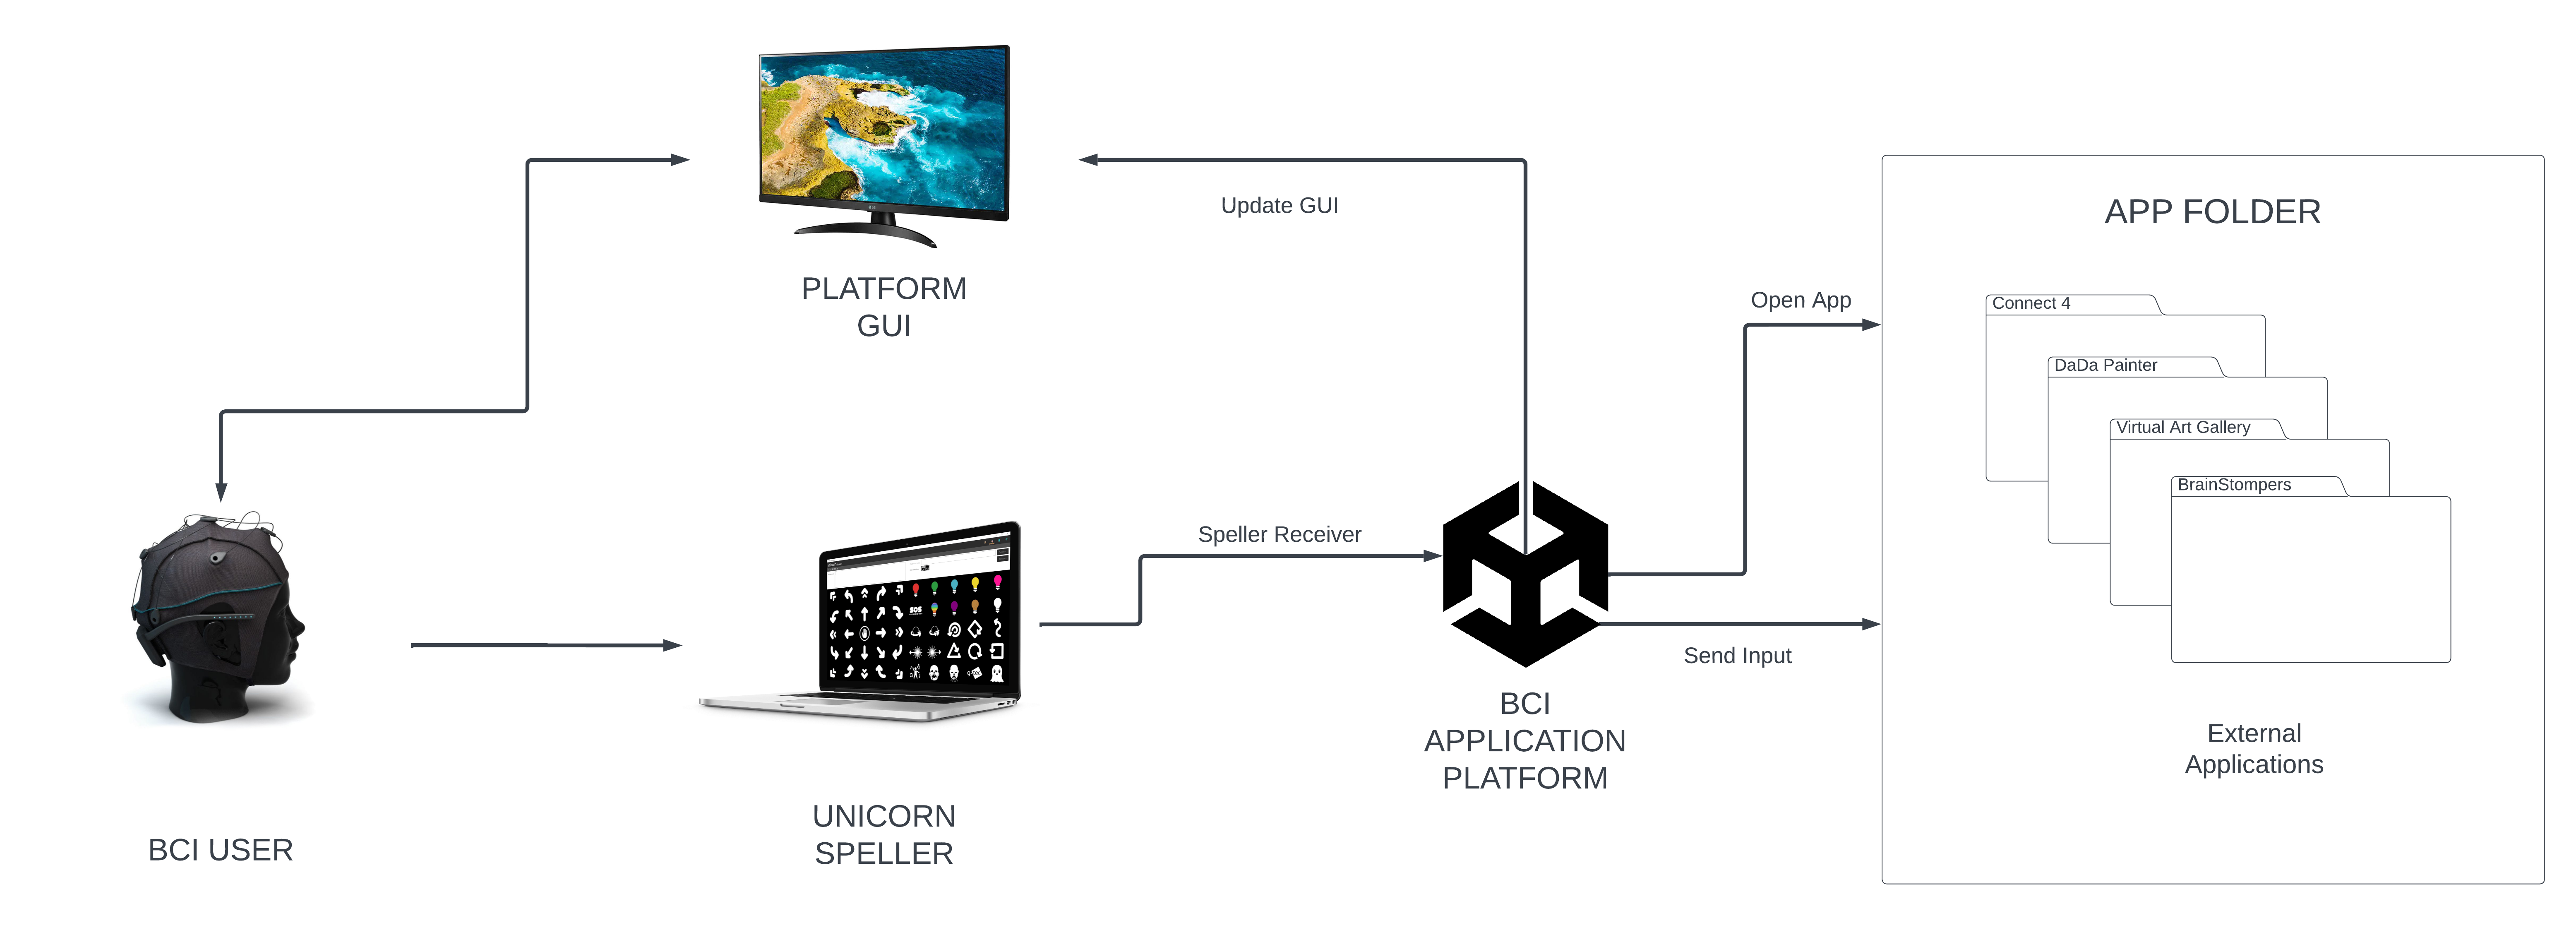
\includegraphics[width=1\textwidth]{Diagrams/Platform Architectural.png}
  \caption{Architectural Diagram}
\end{figure}


\section{Implementation Details}
The Platform is built and run using the Unity Engine and all scripting is done in the C\# programming language. The engine ensures great control over the UI elements on the front end of the application and stability in the back end.

\subsection{Game Objects and UI}
 To display all the applications to the user, they need to be in a centralised location, where the platform can locate them and show them to the user. The location picked for this purpose is inside the User's Documents directory, in a directory called \textit{.bciapps}. Inside here, all applications sit in their separate folder. Furthermore, to automate the platform better, a similar file structure was used between each of the applications, where every application folder contains an \textit{app.exe} file, which is the app executable file called by the platform when the user decides to open that specific app, and another \textit{icon.png} which is that specific application's icon that is being displayed inside the platform to the user. This file structure is reminiscent of other software platforms, such as Steam, which use specific directories to store their applications.
\subsubsection{The App Class}
An App.cs file was created to store all information about a specific application present in the .bciapps folder. This class contains member variables for the application name as well as member variables for both the absolute path of the app's executable file and its icon file. The class also contains a member function called run(), which is used to start the application when the user selects it and decides to do so via Unity's Process.Start() function.
\subsubsection{App Prefabs and Management}
\begin{lstlisting}[language={[Sharp]C}, caption={Manager.cs initialisation}, label={Script}]
void Start() {
    userPath = getUserPath();
    string[] folders = Directory.GetDirectories(userPath);

    string app;
    string icon;
    foreach (string folder in folders) {
        app = folder + "\\app.exe";
        icon = folder + "\\icon.png";
        App newApp = new App(folder, app, icon);
        newApp.debugPrint();
        apps.Add(newApp);
        appCounter++; }
    int xpos = 0;
    foreach (App i in apps) {
        var newObj = GameObject.Instantiate(prefab, new Vector3(xpos, 0, 0), Quaternion.identity);
        byte[] fileData;
        if (File.Exists(i.iconPath)) {
            fileData = File.ReadAllBytes(i.iconPath);
            Texture2D texture = new Texture2D(1, 1);
            texture.LoadImage(fileData);
            Sprite sprite = Sprite.Create(texture, new Rect(0, 0, texture.width, texture.height), new Vector2(0.5f, 0.5f));
            newObj.GetComponent<SpriteRenderer>().sprite = sprite; }
        newObj.transform.parent = container.transform; }}
\end{lstlisting}


An empty game object was created to house Manager.cs, a C\# script used to manage all apps. Another game object, a prefab, is created with a Sprite Renderer. This prefab will serve as the base for all app Game Objects when they get instantiated. 
\vspace{\baselineskip}\newline
Before the main game loop starts, in the Start() function provided by Unity, this script browses the .bciapps directory and for each application, it creates a new App type object which it then stores in a list. The list of apps gets instantiated inside of a container Game Object, with each icon file getting transformed into a Texture2D type, which is then fed to the Sprite Renderer to display the icon to the user[see listing 3.1].

In order to make the UI reflect the change in the user choice, the whole container Game Object in which the application instances are housed is moved with the user's input. This simple approach[see listing 3.2] using a container app makes it easier to instantiate all applications without having to worry about moving each one every time the user changes his/her selection.

\begin{lstlisting}[language={[Sharp]C}, caption={Manager.cs initialisation}, label={Script}]
public void moveContainer(Direction direction)
{
    if(direction == Direction.RIGHT) {
        container.transform.position = new Vector3(container.transform.position.x - 3, 0, 0);
    }
    if(direction == Direction.LEFT) {
        container.transform.position = new Vector3(container.transform.position.x + 3, 0, 0);
    }
}
\end{lstlisting}


\subsection{Speller Board}
 To use the platform, we must first load the custom board \textit{platform.ibc} into the speller. To do so, we simply select the cog menu in the top left of the speller, selecting "Board and timing...". Inside this new window, we click the "Load" button in the bottom left of the window and select the aforementioned .ibc file. As this is part of the initial app setup, this obviously cannot be done by a disabled individual without help. The upside of the Unicorn speller is that once a board is set, the speller always loads the last configuration, so this step is a "set it and forget it" part of the setup.
\vspace{\baselineskip}\newline
To navigate the platform the user must look at one of the navigational buttons on the right side of the speller board. Looking and the left or right arrows, the user can move the app selection to the left or right respectively. Once the desired app is selected the user can open it using the Enter key situated in the center of the navigation buttons. Once the application is open, the same board is used to give input to the individual apps inside the platform. Once an application or program is no longer desired, the X button in the top right-hand side can be used to send a signal to close the app down. This is an item that requires double selection (meaning the user has to select it twice for the app to be closed) to prevent accidental closure of an application. The user may also choose to close the platform itself if he/she so desires employing the use of the same X button. This functionality could have been limited to the applications alone, but I choose against it because the users can utilise this "oversight" to signal a helper or assistant that they no longer wish to continue and want to stop using the application.

\begin{figure}[H]
  \centering
  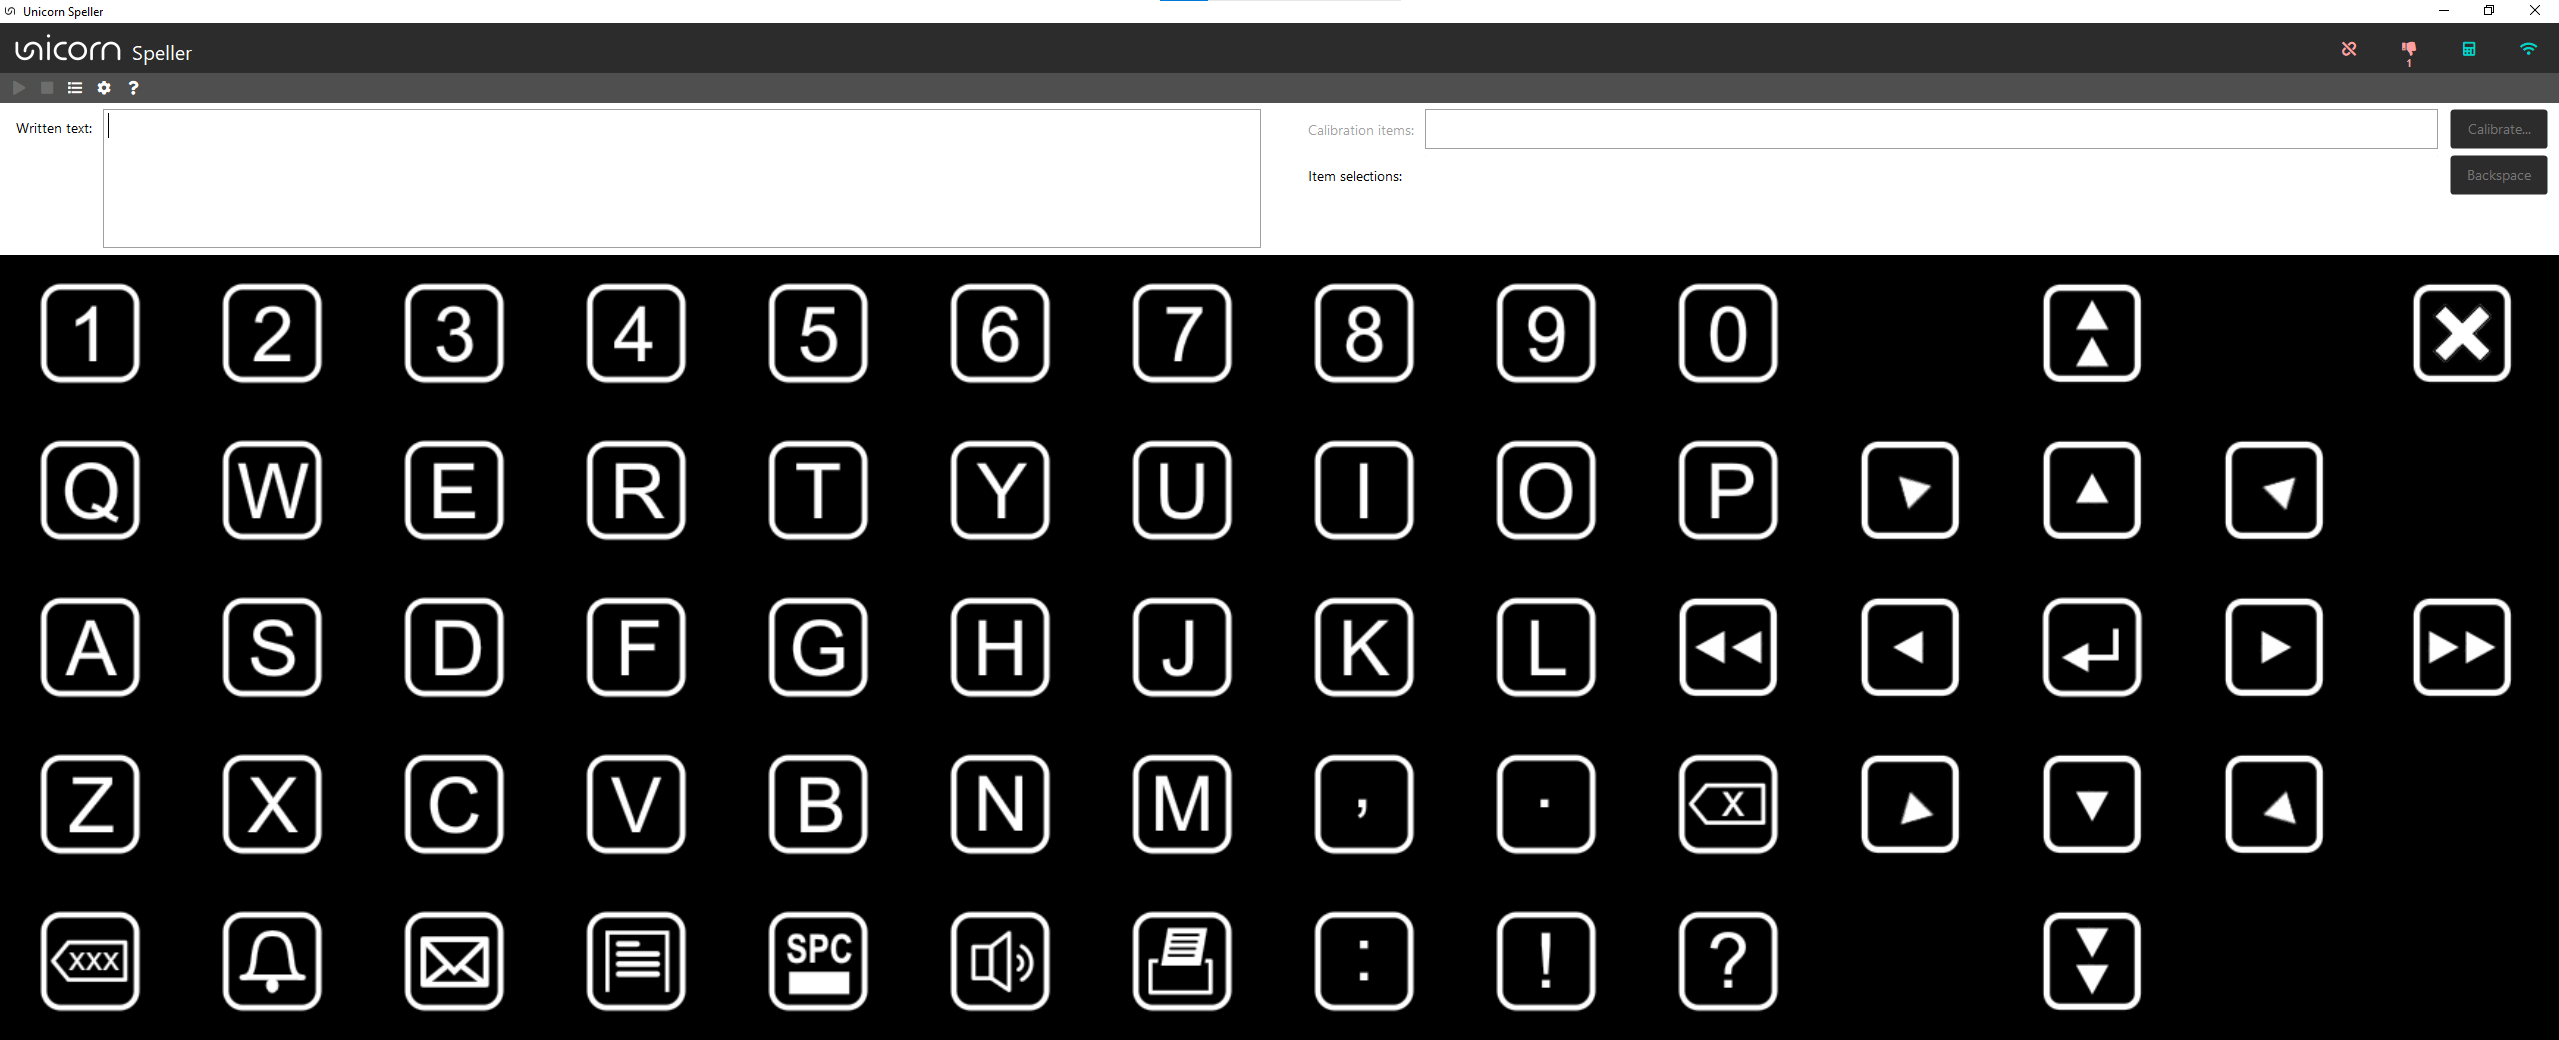
\includegraphics[width=1\textwidth]{Graphics/Platform Custom Board.png}
  \caption{The custom .ibc board used for the platform}
\end{figure}


The Platform speller consists of a full QWERTY-style keyboard and a navigation pad on the right-hand side of the keyboard[see Fig 3.3]. This may seem a bit excessive for a simple platform and that is because it is. The applications inside of the platform use the speller for input as well, all of them implementing their receivers. This would be a non-issue if the board file could be changed during run-time, but it cannot as the speller settings cannot be changed while the speller itself is running. Scripts could be created to automate this, but scripts can fail and in the event of such failure, an able-bodied person would have to step in, which is unsatisfactory. This creates an issue in the implementation where either all apps have to be designed to work with the same style of board (which would mean app integration takes longer, as each app's receiver code needs to be changed) or an umbrella board that covers all bases needs to be created. In this implementation, I have opted to create such a board that covers all needs.


\subsection{Speller Receiver}
The Unicorn Speller outputs via network using UDP. To get the user's input signals, we must implement a UDP port listener that always listens on port 1000 (the default port of output on the speller). The network output of the speller sends a datagram with different data, from the speller version to the different flashing images that the selected item has. The part of the datagram that interests us for this implementation is OutputText. This text field is set inside the board configuration, with each item sending a different output text (eg. the item corresponding to the A letter on the board has the output text also A). As with most board elements, this can be edited. For this implementation, the navigation side of the speller board is given distinctive output text(such as SELECT and ALTF4). Inside the UDP listener, we search the message received through the port for these exact texts[see listing 3.3]. Since the texts are long and unique enough, the risk of finding the exact text inside of a random message is minimal. If one of the text strings corresponding to a command is found inside of the UDP message, the command associated with it is executed inside of the platform. In this way, we can pick up any relevant input from the BCI through the listener function.
\begin{lstlisting}[language={[Sharp]C}, caption={Manager.cs initialisation}, label={Script}]
private string[] navigationCommands = new string[] { "LEFT", "RIGHT", "SELECT", "ALTF4" };

private async void UDPListener() {
    while (inputFlag == true) {
        try {
            var receivedResult = await udpClient.ReceiveAsync();
            string message = Encoding.UTF8.GetString(receivedResult.Buffer);
            foreach (var navCmd in navigationCommands) {
                if (message.Contains(navCmd)) {
                    switch (navCmd) {
                        case "LEFT": {
                                if (selectedApp > 0) shouldMoveLeft = true; }
                            break;
                        case "RIGHT": {
                                if (selectedApp < appCounter - 1) shouldMoveRight = true; }
                            break;
                        case "SELECT": {
                                runSelectedApp(); }
                            break;
                        default:
                            break;
        }}}}
        catch (Exception e) { Debug.LogError($"Exception: {e}"); }
    }
}
\end{lstlisting}


This UDP listener enables the user to interact with the platform by selecting, closing and switching apps. Individual applications will have their own input-catching methods, so this listener is only limited to the application itself, without the need to pass input along to the separate programs housed inside the platform.

\section{Example run}
\subsection{Initial Setup}
Before a disabled user can use the application on their own, an initial setup must be performed with the help of an able-bodied individual. This helper will need to first apply the headset to the head of the disabled person. After that is done, a calibration sequence must be run. It is important to run the sequence with as many flash cycles as possible to ensure the accuracy of the speller during the use of the platform. As mentioned above, the custom board must be loaded to interface with the platform. Other settings the users can tinker with are the duration between flashes, so that the user gets enough time to gaze at the app UI before returning to the speller, the number of flashes per item and the flashing patterns. All these settings are subjective to the user so fine-tuning is necessary.
\subsection{Downloading the Platform and Apps}
After the platform is downloaded or installed[see chapter 4], the user must install applications in the .bciapps file located in \textit{C:$\backslash$Users$\backslash$\%username\%$\backslash$Documents$\backslash$.bciapps}. This can be done either manually or using the installer[see Chapter 4]. For the applications to work with the platform, they must have a specific file layout and have speller boards similar to the one being used in the platform itself.
\subsection{Using the Platform}
The platform can be run through its executable \textit{.exe} file. It is designed to run windowed so that the speller can be run alongside it in a different window, but a second display makes for a better experience. Now the disabled user can run and close apps at his/her leisure, until they get tired or wish to stop, at which point the application and speller, can just be exited out of. This can all be done through the board, and the users must shift their vision from the speller window where the input is taken to the platform UI window where they can see what their inputs are actually doing. This can cause strain in the long run, so monitoring the user's state is an important step throughout use.

